\subsection{Kubernetes as a Docker containers orchestration system}
\textit{This section describes what Kubernetes is and what problems it solves. Furthermore, the section acknowledges Kubernetes popularity and briefly presents chosen Kubernetes objects.}
~\\
~\\
\subsection{Kubernetes architecture}
% this short summary before each section helps me to stay focused on what i want to write about
\textit{This section contains a high level description of the Kubernetes architecture. The focus is on the responsibilities of each Kubernetes component.}
~\\
~\\
\subsubsection{Kubernetes cluster}
A \textbf{Kubernetes cluster} is a single unit of computers which are connected to work together. Any such cluster includes two kinds of instances: masters and nodes. An instance can be a virtual machine or a physical computer. This is depicted on the figure below\footnote{\cite{k8s-cluster}, p. 4}:
\begin{figure}[H]
    \centering
    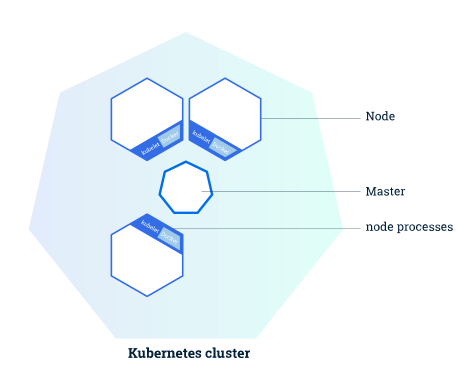
\includegraphics[width=8cm]{figures/cluster.png}
    \label{fig:cluster}
    \caption{Kubernetes cluster diagram}
    \small{Source: https://kubernetes.io/docs/tutorials/kubernetes-basics/create-cluster/cluster-intro/, (accessed: 14.04.2020)}
\end{figure}

\subsubsection{Masters and nodes}
\textbf{The role of the master is to manage the cluster} which means: schedule applications, maintain their desired state, scale them, handle events, manage nodes. \textbf{Nodes serve as the worker machines}. They are responsible for running containers and handling container operations. Masters schedule containers to run on nodes\footnote{\cite{book-mastering-k8s}, p. 5, \cite{k8s-cluster}}. At least one node and one master is needed in a Kubernetes cluster. In order to provide fault-tolerance and high availability in production environments multiple master and multiple node instances are run\footnote{\cite{k8s-components}}.

The instances in a Kubernetes cluster (masters and nodes) are hosts to several \textbf{Kubernetes components}. There are master components, used to control the cluster and there are also node components, run on each node. All the components are presented on the next image:
\begin{figure}[H]
    \centering
    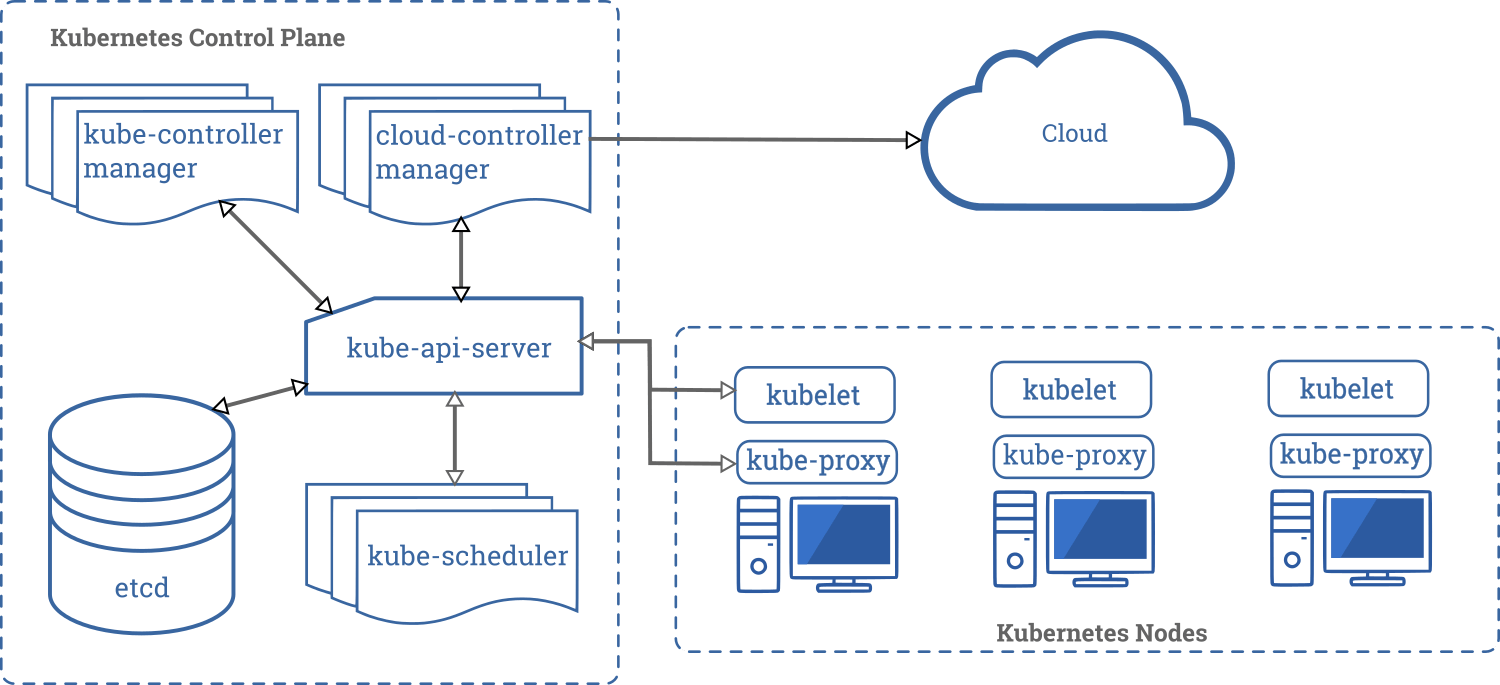
\includegraphics[width=14cm]{figures/components-of-kubernetes.png}
    \label{fig:cluster}
    \caption{Kubernetes components}
    \small{Source: https://kubernetes.io/docs/concepts/overview/components/, (accessed: 14.04.2020)}
\end{figure}


\subsubsection{Components}
The master components are also known as the control plane’s components. Below the master components are itemized\footnote{\cite{book-mastering-k8s}, p. 13,\cite{k8s-components}}:
\begin{itemize}
\item API server
\item Etcd
\item Scheduler
\item Controller manager and Cloud Controller manager
\end{itemize}

\paragraph{}
\textbf{API server} exposes the Kubernetes REST API. It allows the nodes to communicate with the master and it also allows end users to interact with the cluster. Thanks to the fact that API server is stateless and that all its data is stored in Etcd, API server can easily scale horizontally. The main implementation of a Kubernetes API server is kube-apiserver\footnote{\cite{book-mastering-k8s}, p. 13, \cite{k8s-cluster,k8s-components}}.

\textbf{Etcd} stores the entire cluster state. It is a highly-available key-value store. It is enough, for a test Kubernetes cluster, to deploy one instance of Etcd. However, for the purposes of high availability and redundancy, a 3-node or even 5-node Etcd cluster is typical. It is recommended to have a back up plan for the data stored in Etcd\footnote{\cite{book-mastering-k8s}, p. 14, \cite{k8s-components}}.

\textbf{Scheduler} is responsible for assiging containers to nodes. Scheduler selects a node for a container to run on. It considers a range of factors: resource requirements, various constraints, affinity and anti-affinity specifications, data locality, inter-workload interference, and deadlines. The implementation is known as kube-scheduler\footnote{\cite{book-mastering-k8s}, p. 14, \cite{k8s-components}}.

\textbf{Controller manager} runs controller process such as: watches the shared state of the cluster and makes changes needed to move the current state into the desired state. Controller manager is a collection of separate managers, but they are all compiled into a single binary and run in a single process in order to reduce complexity. The controllers consist of: Node Controller, Replication Controller, Endpoints Controller, Service Account and Token Controllers. The implementation of Controller manager is kube-controller-manager\footnote{\cite{book-mastering-k8s}, p. 14, \cite{k8s-components}}. \textbf{Cloud Controller manager} interacts with a specified underlying cloud provider (e.g. Amazon Web Services or Google Cloud Platform). It allows the Kubernetes code and the cloud vendor’s code to evolve independently. It is implemented by cloud-controller-manager\footnote{\cite{k8s-components}}.

As aforementioned, there are also node components. They run on both: masters and nodes. They are listed below\footnote{\cite{book-mastering-k8s}, p. 13,\cite{k8s-components}}:
\begin{itemize}
\item Kubelet
\item Proxy
\item Container Runtime
\end{itemize}

\paragraph{}
\textbf{Kubelet} oversees the communication with the master components (by monitoring API server for changes) and makes sure that containers, described by a Pod, are running and healthy (so it manages a Pod lifecycle). A Pod is a simple object from a Kubernetes API and it represents a set of containers. Containers which were not created by Kubenernetes are not managed by Kubelet\footnote{\cite{book-mastering-k8s}, p. 15, \cite{k8s-components}}.

\textbf{Proxy} is implemented by kube-proxy. It is a network proxy and it implements a part of the Kubernetes Service concept, which means that it is responsible for exposing an application as a network service and it provides load balancing\footnote{\cite{book-mastering-k8s}, p. 247, \cite{k8s-components}}.

\textbf{Container Runtime} is the software which is responsible for operating containers. Several container runtimes are supported: Docker, containerd, CRI-O, and any implementation of the Kubernetes CRI (Container Runtime Interface). It is a design policy of Kubernetes that is ought to be decoupled from a specific container runtime. Under some circumstates it should be possible to switch from one container runtime to another or to use multiple of them at once. Originally, Kubernetes was designed to manage only Docker containers\footnote{\cite{book-mastering-k8s}, p. 15, \cite{k8s-components}}.

\subsubsection{Other services}
Apart from master and node components, there are also \textbf{add-ons, extensions, and third party tools} which communicate with Kubernetes by the API server and which provide additional functionality. Examples of such services are: DNS, Vertical Pod Autoscaler, Cluster Autoscaler, Istio, Kubernetes Dashboard, kube-ops-view, node-problem-detector, etc\footnote{\cite{book-cndwk}, p. 12, 84, 102, 175}}.

TODO: describe such of them which will be used later.

\subsubsection{The Kubernetes networking model}
Kubernetes states a few \textbf{networking requirements}\footnote{\cite{k8s-net}}:
\begin{itemize}
\item pods on a node must be able to communicate with all pods on all nodes without Network Address Translation (NAT)
\item agents on a node (e.g. system daemons, kubelet) must be able to communicate with all pods on that node
\end{itemize}

There are many available options that help with satisfying these requirements, e.g.: AWS VPC CNI for Kubernetes, Azure CNI for Kubernetes, Flannel, OpenVSwitch, Project Calico, etc\footnote{\cite{k8s-net}}. CNI stands for Container Networking Interface and it is a specification and also a set of libraries for writing network plugins to configure network interfaces in Linux containers. A CNI container is bound to have its own IP address. For Kubernetes, \textbf{each pod has its own IP address}, so the pod is the CNI container\footnote{\cite{book-mastering-k8s}, p. 254, 255}. \textbf{Containers that belong to a one pod share the same IP address}, which means that these containers can reach all reach each other’s ports on localhost and also that none two containers should expose the same port. This model is known as "IP-per-pod"\footnote{\cite{k8s-net}}.

TODO: AWS VPC CNI for Kubernetes or Flannel? describe such of them which will be used later.
